% Tento soubor nahraďte vlastním souborem s obsahem práce.
%=========================================================================
% Autoři: Michal Bidlo, Bohuslav Křena, Jaroslav Dytrych, Petr Veigend a Adam Herout 2019

% Pro kompilaci po částech (viz projekt.tex), nutno odkomentovat a upravit
%\documentclass[../projekt.tex]{subfiles}
%\begin{document}

\chapter{Úvod}
\label{uvod}
Tato bakalářská práce je věnována návrhu a implementaci digitálního záznamníků s autonomním dokončením záznamu dat při výpadku napájení. Požadavek na zařízení vznikl od firmy NXP Semiconductors, 
konkrétně od týmu zaměřeného na bezdrátové nabíjení, ve kterém pracuji. Tento tým působí v České republice, jak v Rožnově pod Radhoštěm tak i v Brně a zároveň má své zastoupení v Asii a Severní 
Americe. NXP Semiconductors je jedním z předních členů WPC (Wireless Power Consortium), organizace zodpovědné za definování standardu Qi pro bezdrátové nabíjení. Primární zaměření NXP v této 
oblasti spočívá ve vývoji referenčních designů pro automotive sektor, kde zákazníkům poskytuje řešení určená pro integraci do vozidel.

Zákazníci, kteří využívají referenční designy NXP, pocházejí z celého světa a dostávají téměř hotový produkt, který lze následně certifikovat v Qi certifikačních laboratořích. Nicméně i přesto, 
že jsou referenční designy navrženy podle nejnovějších standardů, často dochází k jejich úpravám podle specifických požadavků zákazníků, zejména s ohledem na konkrétní poptávku koncového 
zákazníka (OEM – Original Equipment Manufacturer). Tyto požadavky jsou obvykle shrnuty v RFP (Request for Proposal), kde zákazník specifikuje konkrétní požadavky na systém. Tyto úpravy mohou 
být například realizovány z důvodu snížení ceny nebo zlepšení výkonu, například EMC charakteristik a nebo speciální chování bezdrátové nabíječky v krajních situacích. 

Při jakýchkoli úpravách však vznikají nové technické výzvy, a proto NXP poskytuje zákazníkům plnou technickou podporu až do úspěšné certifikace. Certifikace probíhá v různých laboratořích po 
celém světě, avšak ne vždy může být přítomen zaměstnanec NXP, který by dohlížel na celý proces a zajistil, že certifikace proběhne hladce. V těchto případech se momentálně tým pro bezdrátové 
napájení spoléhá pouze na záznamy poskytnuté operátorem certifikační laboratoře. Tyto záznamy však pocházejí pouze ze strany přijímače – tedy certifikačního zařízení, zpravidla od výrobců Nok9 
nebo Granite River Labs (GRL). Ty poskytují některé z důležitých informací, bohužel tyto nabídnuté záznamy nezahrnují explicitní informace o chování vysílače. Pokud tedy bezdrátová nabíječka, 
tedy vysílač nějakým testem neprojde, což se občas stává, je často náročné zpětně identifikovat příčinu problému. \cite{nxp_wireless_charging_team}

Nezbytným požadavkem na implementaci tohoto záznamníku je i jeho snadná obsluha, neboť zařízení bude poskytováno zákazníkům pro účely certifikace. V klasickém scénáři zákazník předá nabíječku 
i se záznamníkem operátorovi certifikační laboratoře, ten si ji připojí k testovanému zařízení. Po skončení testovacího dne operátor záznamník vrátí zákazníkovi, který jej následně připojí 
k počítači a odešle společnosti NXP Semiconductors získané záznamy.


\chapter{Záznam dat}
\label{zaznam_dat}

\label{uvod}

\section{Počátky záznamu a zpracování dat (Historie záznamu a zpracování dat - předchozí název)}
\label{historie}
Lidstvo již od svých počátků potřebovalo zaznamenávat data, neboť člověk mnohdy dokáže datům přiřadit sémantiku - tedy význam, a proměnit je tak v informace. Právě díky nim se lidé mohou učit 
z minulých zkušeností, předávat znalosti dalším generacím, organizovat společenské a obchodní procesy a podporovat rozvoj vědy a technologií. Proto se již od pravěku hledaly způsoby, 
jak evidovat důležité události a hodnoty. První formy záznamu dat sahají až do doby 19 tisíc let před Kristem, kdy v paleolitu vznikl nástroj známý jako kost Ishango. Tento jednoduchý nástroj, 
vyrobený z kosti paviána, obsahoval vyryté zářezy, které pravděpodobně sloužily k provádění základních matematických operací, jako je sčítání či násobení.

\begin{figure}[h] % obrazek ishango
    \centering
    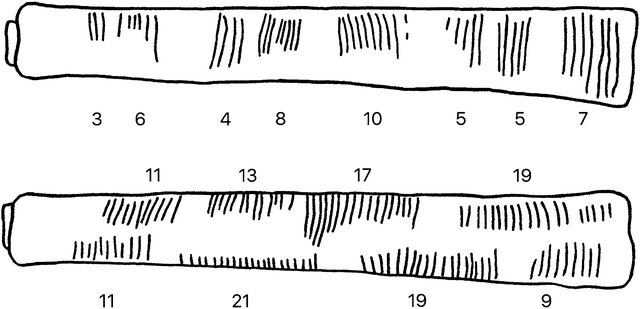
\includegraphics[width=0.6\textwidth]{obrazky-figures/ishango.jpg}
    \caption{Kost Ishango sloužící k záznamu informací v době Paleolitu \cite{ishango_picture}}
    \label{fig:ishango}
\end{figure}

S příchodem prvních civilizací se začaly vyvíjet lepší metody uchovávání dat. Ve starověké Mezopotámii, v oblasti mezi řekami Eufrat a Tigris, kde sídlil národ Sumérů, vzniklo kolem roku 3400 
před naším letopočtem klínové písmo. Tento typ písma byl využíván hlavně pro zápis obchodních transakcí, zákonů a dalších důležitých informací, které byly zaznamenávány na hliněné tabulky 
pomocí rákosového stylusu. O několik století později, kolem roku 3200 př. n. l., začali Egypťané používat hieroglyfy, které byly ryty do kamene nebo zapisovány na papyrus, což umožnilo 
uchovávat důležité administrativní a náboženské záznamy. V Číně se mezi 1200–1000 př. n. l. používaly věštecké kosti, na které se zaznamenávaly otázky kladené orákulu - což jsou důležité 
otázky, zejména ve věcech budoucnosti, i jeho odpovědi, čímž vznikly první organizované záznamy psané ranými čínskými znaky.

\newpage

Průlomem pro zaznamenáváním dat, bylo vynalezení knihtisku, které vymyslel Johann Gutenberg ve 40. letech 15. století. Do této doby byly informace zaznamenávány ručním přepisováním, což 
bylo zdlouhavé a nákladné. V počátcích měl knihtisk význam převážně z náboženského hlediska, díky tisku se Bible mohla šířit mezi širokou veřejností, což přispělo k protestantské reformaci a 
změně křesťanského světa. Nicméně knihtisk obecně změnil způsob, jakým lidé přistupují k informacím a učinil je dostupnějšími. \cite{knihtisk_medium}

V 17. století se dále pokročilo, jak v způsobech záznamu dat, tak i s jejich zpracováním. Významným představitelem tohoto období je John Graunt, jež se věnoval studiu dat o úmrtnosti v Londýně, 
během čehož odhalil určité opakující se vzorce a zákonitosti na základě, kterých položil základy moderní statistiky. V následujících staletích pokračoval vývoj metod pro práci s daty, zejména 
díky rozvoji matematiky, fyziky a statistiky. \cite{britanicca_John_Graunt}
% Jako hlavni predstavitele tohoto obdobi lze uvest jmena jako Bayes, Laplace, Pierre-Simon, Carl Friedrich Gauss, Galton
\section{Záznam a zpracování dat v moderní době}
% TODO: pocet normostran (cca 3.1)
S pokročilými metodami na zpracování dat, také rostly nároky na výpočty a vznikla tak potřeba efektivnějších nástrojů pro zisk a analýzu dat. S tímto rozvojem souvisí i technologický pokrok v 
oblasti záznamu dat, který prošel dlouhou cestou – od jednoduchých mechanických přístrojů přes magnetické pásky až po moderní digitální záznamníky schopné uchovávat a analyzovat obrovské objemy 
informací v reálném čase.

%\section{Možnosti záznamu dat}
%\label{moznosti_zaznamu_dat}
  
\subsection{Analogový záznam dat} %TODO: zde popsat i analogový záznam i digitální záznamníky
\label{moznosti_zaznamu_dat}
Prvními specializovanými záznamníky byly mechanické či elektromechanické zařízení, využívající principu analogového záznamu dat. Jejich primárním účelem bylo zaznamenávání fyzikálních veličin, 
jako je například teplota, tlak, vlhkost nebo vibrace. Tyto přístroje využívaly myšlenky mechanického pohyblivého pera, které převádělo naměřenou hodnotu fyzikální veličiny na samočinný pohyb. 
Pro realizaci tohoto pohybu bylo nutné nejprve převést měřenou fyzikální veličinu na mechanický posun. Například pro měření teploty se běžně využíval bimetalový pásek, složený ze dvou kovových 
materiálů s různou hodnotou teplotní roztažitelnosti. Při změně teploty docházelo k prohnutí pásku v důsledku rozpínání kovu, čímž se rozpohybovalo mechanické pero, které zapsalo hodnotu na 
paměťové médium. 

% mechanicky -< samocinny
% pomocí kterého se zapisovala změřená hodnota na paměťové médiu (papírová páska nebo papírový buben)

\begin{figure}[h] % obrazek polygraf
    \centering
    \includegraphics[width=0.50\textwidth]{obrazky-figures/polygraaf.png}
    \caption{Ukázka zařízení patřící do skupiny analogových záznamníků - polygraf \cite{polygraph_picture}}
    \label{fig:polygraaf}
\end{figure}


Tyto přístroje byly běžně používány od 19. století. Pro již zmíněný záznam teploty se využíval například přístroj zvaný cirkulární grafový záznamník (Circular Chart Recorder), dále byl hojně 
využíván polygraf, využívaný jako detektor lži. Značnou nevýhodou těchto záznamníků byl typ paměťového média, na které probíhal zápis hodnot, nejčastěji jim byla papírová páska nebo papírový 
buben. Tyto pásky musely být velice často měněny za ještě nepopsané, jelikož výsledné záznamy by se staly značně nepřehledné, pokud by byly popsány vícekrát.
Další limitací těchto přístrojů bylo ruční vyhodnocování dat, což bylo mnohdy časově zdlouhavé a také náchylné k chybám. K správné interpretaci dat byla často potřeba zkušená obsluha a v 
některých případech i pomocné měřící pomůcky. Přenos souborů a automatizace také nebyla možná, proto jakmile se dostaly v polovině 20. století na trh číslicové systémy, začal 
jejich úpadek. \cite{newcastle_history_of_digital_computers, florian_prechod_a_analog_do_digital}

Jak obecne probiha princip digitalniho zaznamu dat, co jsou to digitalni data, ze se v dnesni dobe uprednostnuje tento zpusob misto analogoveho zaznamu.

% TODO: Kde napsat co je to vubec zaznamnik? Ze je to pristroj, ktery zpracovava, uklada a pripadne analyzuje data...
\section{Digitální záznam dat}
\label{digitalni_zaznamnik}
Co je to digitální záznamník + jak zaznamnik realizovat jestli PC nebo MCU (dedikovane zarizeni). Historie - odkdy se zacinaly pouzivat cislicove (digitalni) systemy, rozdily v zaznamu 
analogovych/digitalních dat

\begin{figure}[h] % obrazek polygraf
    \centering
    \includegraphics[width=0.95\textwidth]{obrazky-figures/common_digital_datalogger_scheme.png}
    \caption{Obecné schéma digitálního záznamníku}
    \label{fig:polygraaf}
\end{figure}
vstupy -> surové data (raw data)

vystupy -> organizovaná data např. v textové podobě

\subsection{Digitální záznam v počítačovém systému}
Ze je to pouze SW implementace zaznamniku, cilem je vyvinout pouze aplikaci pro zaznam dat, lze vybirat z daleko vice jazyku, K cemu jsou vyuzivany digitalni zaznamniky na PC.

\subsection{Digitální záznam na platformě mikrořadiče}

\section{Koncepty využívané ke zpracování dat digitálních záznamníků}
What is Lorem Ipsum?
Lorem Ipsum is simply dummy text of the printing and typesetting industry. Lorem Ipsum has been the industry's standard dummy text ever since the 1500s, when an unknown printer took a galley of type and scrambled it to make a type specimen book. It has survived not only five centuries, but also the leap into electronic typesetting, remaining essentially unchanged. It was popularised in the 1960s with the release of Letraset sheets containing Lorem Ipsum passages, and more recently with desktop publishing software like Aldus PageMaker including versions of Lorem Ipsum.

Why do we use it?
It is a long established fact that a reader will be distracted by the readable content of a page when looking at its layout. The point of using Lorem Ipsum is that it has a more-or-less normal distribution of letters, as opposed to using 'Content here, content here', 

\subsection{Vícenásobná vyrovnávací paměť (multiple-buffering)}
Jedním z častých konceptů využívaných v implementaci digitálních záznamníků je použití vícenásobné vyrovnávací paměti. Tento koncept je převážně známý díky algoritmům využívaným v oboru 
počítačové grafiky. Grafický čip musí zpracovat velké množství dat za krátký časový úsek, proto algoritmus zpracování dat využívá dvě vyrovnávací paměti - přední vyrovnávací paměť, takzvaný 
front-buffer, jež je využívána pro zobrazení aktuálního snímku a zadní vyrovnávací paměť, ve které čip připravuje nový obsah. Výsledný obsah tak může být plynule vykreslen bez artefaktů a 
trhání. Jakmile je nový snímek kompletní, vyrovnávací paměti se prohodí. \cite{double_buffering_model}

Obdobný mechanismus se využívá i v digitálních záznamnících, kde slouží k zajištění kontinuálního sběru dat bez výpadků. Zatímco jeden buffer přijímá nová data ze vstupní periferie 
(například analogově-digitálního převodníku či jiných vstupů), druhý buffer je současně zpracováván nebo ukládán na úložné médium. Tím se minimalizuje riziko ztráty dat způsobené časovou 
prodlevou při jejich zpracování nebo zápisu.

\begin{figure}[h]
    \centering
    \includegraphics[width=0.95\textwidth]{obrazky-figures/multiple_buffering-1.png}
    
    \caption{Schéma principu práce s vícenásobnou vyrovnávací paměťí - náhodný stav}
    \label{fig:multiple-buffering-1}
\end{figure}

Důležitou vlastností tohoto algoritmu je jeho nízká operační režijní náročnost. Plynulý chod zpracování dat je zajištěn bez nutnosti fyzického přenosu obsahu mezi vyrovnávacími pamětmi. 
Místo toho se využívají ukazatele (pointery), které směřují na počáteční adresy jednotlivých bufferů. Jakmile je sběrný buffer (Back Buffer) naplněn, ukazatele se prohodí~–~back buffer se 
stane zpracovávaným bufferem (Front Buffer) a původní front buffer se uvolní pro další sběr dat.

\begin{figure}[h]
    \centering
    \includegraphics[width=0.90\textwidth]{obrazky-figures/multiple_buffering-2.png}
    
    \caption{Schéma principu práce s vícenásobnou vyrovnávací paměťí - přeřazení ukazatelů}
    \label{fig:multiple-buffering-2}
\end{figure}

Tato metoda nachází významné uplatnění zejména v systémech pracujících v reálném čase, kde dochází k příjmu velkého objemu dat v krátkých časových intervalech a kde doba zpracování nesmí 
překročit dobu sběru dat. Využitím vícenásobné vyrovnávací paměti se minimalizuje latence zpracování a současně se snižuje riziko přetečení paměťového prostoru. \cite{buffering_chang}

Nicméně, žadný algoritmus není dokonalý a i tato metoda mé své nevýhody, které je třeba zmínit. Vyrovnávací paměti jsou zpravidla implementovány softwárově, nikoliv hardwarově, což vede 
k zvýšeným nárokům na paměťové prostředky, obzvlášť v segmentu volatilní paměti (SRAM/DRAM) kde jsou buffery uložené. \cite{basics_of_digital_forensics}
% TODO: Je tedy vhodne si promyslet zda zdroje MCU budou dostacovat.

\subsection{Dávkové zpracování (batch processing)}
Další princip, jež je využívaný v implementacích digitálních záznamníků, souvisí s typem uložišť na které jsou získaná data zaznamenávána. Některé typy nevolatilních pamětí, například 
NAND Flash paměť, jež umožňují uchování dat i po odpojení napájení. Tyto druhy paměti jsou organizovány do bloků (viz. obrázek \ref{fig:batch-processing}), přičemž bloky jsou následně 
rozděleny na menší jednotky zvané sektory. Velikost sektoru obvykle bývá 512 bajtů či 4096 bajtů, v závislosti na typu média a jeho architektůře. Tato bloková struktura, umožňuje účinnou 
správu prostoru, které uložiště nabízí, ale současně vyžaduje specifický způsob zápisu/čtení dat, které je pouze umožněno na úrovni celých bloků.  \cite{tech_target_nand_flash, non_volatile_memories}

Dávkové zpracovátí tohoto chování paměti využívá, data se tedy nejprve shromažďují ve volatilní paměti - například RAM a teprve po naplňení určitého objemu (celého bloku či jeho násobku) 
dojde k jejich zápisu na konečné paměťové médium.

\begin{figure}[h]
    \centering
    \includegraphics[width=0.70\textwidth]{obrazky-figures/batch_processing.png}
    
    \caption{Organizace nevolatilní paměti}
    \label{fig:batch-processing}
\end{figure}


\subsection{Cirkulární buffer}
Cirkulární buffer (circular buffer), někdy označovaný také jako kruhový nebo cylindrický buffer, je datová struktura, která funguje na principu kruhové fronty (FIFO – First-In, First-Out). 
Tento přístup je často využíván v systémech pro zpracování datových toků, jako jsou digitální záznamníky, kde je nezbytné kontinuálně přijímat data bez přerušení či ztráty vzorků.


\begin{figure}[h]
    \centering
    \includegraphics[width=0.60\textwidth]{obrazky-figures/circular_buffer.png}
    
    \caption{Cirkulární vyrovnávací paměť}
    \label{fig:circular-buffer}
\end{figure}

\newpage

Princip činnosti cirkulárního bufferu spočívá v použití dvou ukazatelů - head (zápisový ukazatel) a tail (čtecí ukazatel). Ukazatel head vždy směřuje na pozici, kam bude zapisován následující 
prvek, zatímco ukazatel tail ukazuje na pozici, ze které bude načtena následující hodnota. Pokud ukazatel head dosáhne konce pole, vrací se na jeho začátek, čímž je zajištěna kruhová povaha 
struktury. Při plném bufferu lze zvolit dvě strategie – přepsání nejstarších dat nebo odmítnutí nových vstupů, přičemž výběr závisí na konkrétní 
aplikaci.\cite{embedjournal_ring_buffer, medium_ring_buffer}

Z hlediska časové složitosti nabízí cirkulární buffer konstantní časovou složitost (O(1)) pro všechny základní operace, jako je zápis (enqueue) a  čtení (dequeue). Tato efektivita je dána tím, 
že se při zápisu a čtení dat není potřeba přesouvat prvky v paměti, ale stačí pouze inkrementovat ukazatele s využitím operace modulo. Pokud jde o prostorovou složitost, velikost cirkulárního 
bufferu je určena předem – zpravidla jde o staticky alokované pole o velikosti n prvků, což odpovídá složitosti O(n), kde n je maximální počet prvků, které může buffer pojmout. 
\cite{petrungaro_ring_buffer_complexity}

\subsection{Nízko-energetické režimy (low-power modes)}
Energetická efektivita je jedním z klíčových parametrů obecně vestavěných zařízení, tedy i digitálních záznamníků implementovaných na platformě MCU, zejména pokud jsou napájeny z baterií či 
jiných omezených zdrojů energie. Minimalizace spotřeby je v těchto případech realizována využitím nízkoenergetických režimů (low-power modes), které umožňují zařízení přejít do stavu s 
minimální energetickou náročností během nečinných period. V praxi mnoho digitálních záznamníků nemusí provádět měření a záznam dat nepřetržitě. Například záznamník teploty může v pravidelných 
intervalech provést měření, uložit naměřenou hodnotu, přejít do režimu nízké spotřeby a po uplynutí definovaného časového intervalu nebo při vyskytnutí speciální události přejít do aktivního 
režimu. \cite{analog_devices_low_power_modes}

Průběh takového cyklického chování spotřeby mikrokontroléru, kde se střídají fáze měření a spánku s pravidelnou periodou měření teploty, je znázorněn na obrázku \ref{fig:low-power-modes} níže.

\begin{figure}[h]
    \centering
    \includegraphics[width=0.90\textwidth]{obrazky-figures/low_power_modes.png}
    
    \caption{Graf znázorňujíci dynamiku spotřeby mikrokontroléru v průběhu času při využití aktivního a nízkoenergetického režimu}
    \label{fig:low-power-modes}
\end{figure}

Ačkoliv nízkoenergetické režimy přinášejí značné úspory energie a jsou nezbytné pro zařízení napájená z baterií, u dataloggerů s velkým objemem zaznamenávaných dat mohou představovat 
významná omezení. Tyto režimy sice snižují energetickou náročnost systému, avšak zároveň omezují schopnost mikrokontroléru rychle reagovat na události. Spánkové stavy, které minimalizují 
spotřebu energie, často vedou k delšímu zpoždění při probuzení a nižší dostupnosti kritických periferií. V aplikacích, kde je vyžadována okamžitá odezva na externí podněty nebo nepřetržité 
zpracování velkého množství dat, může tento faktor negativně ovlivnit spolehlivost a efektivitu záznamníku. \cite{embedded_low_power_modes}

V těchto případech je proto vhodné zvážit provozní podmínky a očekávanou dostupnost systému. Pokud záznamník pracuje s velkým datovým tokem a má možnost být po dobu záznamu stále dostupné 
externí napájení, může být výhodnější upustit od implementace nízkoenergetických režimů a místo toho optimalizovat architekturu systému pro nepřetržitý provoz s důrazem na výkon a rychlou 
odezvu. \cite{analog_devices_low_power_modes}

\section{Typy médií pro záznam dat}
Hard disk, vyhody nevyhody,... 

\chapter{Návrh digitálního záznamníku}

\section{Existujících řešení digitálních záznamníku}

\section{Výběr vhodné platformy}
Neni vhodne implementovat zaznamnik na pocitacovem systemu, je treba zvolit stragii implementace na mikroradici, porovnat FRDM-MCXN947, Arduino, Raspberry
\subsection{FRDM-MCXN947}

\subsection{Arduino}

\subsection{Linux based - Raspberry}

Pripraven i popis jadra ARM Cortex-M33, ktere vyuziva FRDM-MCXN947.

% ----------------------------------------------------
% DALSI NAZVY: Volba datového úložiště, Výběr externího uložiště pro záznam dat, Možnosti způsobu ukládání získaných dat
\section{Přístupy k ovládaní úložiště}
Obecný popis, proč je potřeba externí uložiště, že by se data mohla ukládat i v RAM paměti, ale že by tam moc dlouho nevydržela, 

\subsection{SDHC}

\subsection{SPI}
\subsection{Quad-SPI flash}


% ----------------------------------------------------
% DALSI NAZVY: Volba datového úložiště, Výběr externího uložiště pro záznam dat
\section{Možnosti správy dat - souborové systémy} 
Obecný popis, souborový systém je zodpovědný za organizaci, správu a přístup k datům na zvoleném úložném médiu.

\subsection{FATFS}

\subsection{Chan FATFD}

\subsection{LittleFS}


% ----------------------------------------------------

\section{Výběr řízení přístupu k získaným datům}

\subsection{USB Mass Storage}

\subsection{Media Transfer Protocol}

\subsection{Human Interface Device}

% ----------------------------------------------------
\section{Výběr zdroje času}

\subsection{Obvod reálného času}

\subsection{Interní časovač}

\subsection{Bezdrátová komunikace (GPS/NTP)}

% ----------------------------------------------------
\section{Výber přístupu řízení běhu aplikace}
Srovnani obecne bare-metal a RTOS.


\subsection{Bare-Metal}

% TODO: Zde to asi spis rozdelit na Baremetall vs. RTOS a pak uvest priklady jako FreeRTOS a ZephyrRTOS
\subsection{RTOS}
\subsubsection{FreeRTOS}
Konkretní výhody a nevýhody FreeRTOS

\subsubsection{ZephyrRTOS}
Konkretní výhody a nevýhody ZephyrRTOS

% ----------------------------------------------------

\section{Architektura systému digitálního záznamníku}
Popis architektury na základě vybraných komponent. Popis blokového diagramu.

% ----------------------------------------------------

\section{Volitelné rozšíření}
\subsection{Měření teploty}

% ----------------------------------------------------

\subsection{Řešení problému synchronizace času}

% ----------------------------------------------------

\chapter{Realizace hardwaru}
Popis co všechno je již na platformě FRDM MCXN947, z toho ti vyplyne co všechno bude ještě muset nabízet expanzní deska.
\section{Základová deska}
\section{Expanzní deska}

\section{Mechanická část}
Jak jsem měřil spotřebu, jak jsem spočítal hodnoty kondenzátorů

\chapter{Softwárová implementace}

\section{Záznamové vlákno}

\section{USB Mass Storage vlákno}

\section{Signalizace stavu systému}

% ==================================================== 
\chapter{Testování systému}
Obecne proc je potreba testovat, jake jsou moznost testovani a validace vestavenych systemu

% ----------------------------------------------------

\section{Testování a validace}

\subsection{Funkcionální testování}
Popis skriptů pro automatické testování, popis výsledků, atd, ...

\subsection{Kontrola bezpečnosti kódu}
MISRA

% ----------------------------------------------------

\section{Limitace systému}
\label{limitace}

% ----------------------------------------------------

\section{Možná rozšíření záznamníku}
\label{mozne_rozsireni}

\chapter{Závěr}
\label{zaverPrace}


%===============================================================================

% Pro kompilaci po částech (viz projekt.tex) nutno odkomentovat
%\end{document}
